\documentclass{article}

\usepackage{fullpage}
\usepackage{amsmath}
\usepackage{amssymb}
\usepackage{tikz}

\begin{document}

\section{Accuracy and Repeatability}

Why is accuracy less than repeatability?

\paragraph{}
Accuracy is generally defined as 
	\emph{how close the manipulator can come to a given
		point in its workspace}.
Note that this point is \emph{described by the operator}.
It has to be given coordinates within the robot's internal
	reference frame for the robot to know where the point is.
Therefore, the accuracy of a robot combines two sources of error:

\begin{enumerate}
\item Differences between the operator coordinate system
	and robot coordinate system due to measurement error in 
	setting up the robot system.
\item Movement errors within the robot coordinate system.
\end{enumerate}

In contrast, the repeatability, which is usually defined as
	\emph{how close a manipulator can return to a previously
		taught point},
	eliminates the first source of error.
The point may have different descriptions in our coordinate system
	and the robot's coordinate system.
However, during the teaching, the operator verified that the point
	in the robot coordinate system corresponds perfectly with the
	point the operator desired it to be.
Therefore, error can only come from the robot failing to move perfectly
	to the point that it intends to move to.

For a robot to be accurate, however, the operator must describe
	the point in the robot's frame, so that the robot intends
	to move where the operator intends it to move.
It is this additional step which makes accuracy more difficult
	than repeatability.

\section{Improving accuracy with Sensing}

How could manipulator accuracy be improved with endpoint sensing?
What difficulties might endpoint sensing introduce into the control
	problem?

\subsection{Improving accuracy with Endpoint Sensing}

Endpoint sensing refers to placing sensors on the end-effector of 
	a robot manipulator in order to give it information about
	what it is doing.

These sensors might addess problem (1) above.
Let's think of an example.

Suppose a robot manipulator is trying to grasp a fork.
The operator will measure the pose of the fork, convert that pose
	measurement in their frame into a position measurement in the
	robot's frame, and then instruct the robot to grasp
	a fork at the desired pose.

If the robot lacks endpoint sensors, all it can do is grasp as if
	there is a fork at the desired point, bindly trusting the operator.
However, if the robot has endpoint sensors, it can compare the 
	instructions with what it senses itself.
As the manipulator approaches the fork, it will be able to make 
	more accurate measurements with its endpoint sensor.
The closer the robot gets, the more it should trust its endpoint
	sensors over the operator data.
This improves accuracy because it allows new measurements of the location
	of the specific point in the robot's frame, which let it get
	more information.
This can all be summarized in the Bayesian formalism by using the user-
	provided data as a prior, and updating the distribution of beliefs
	in poses with its measurements.
Endpoint sensing addresses the description error mentioned in part
	(1), because it uses sensors to make sure that the robot's intended
	target isn't far off from the real-world target.

\subsection{Additional Difficulties from Endpoint Sensing}

Endpoint sensing brings with it additional difficulties.
Without endpoint sensing, the control problem is merely moving from
	one point in manipulator state space to another.
Once endpoint sensing is introduced, however, one has to either
	stop the manipulator with each measurement,
	or make the measurements while the manipulator is moving and then
	retarget the manipulator on the fly.
Stopping the manipulator with each measurement would be much slower,
	and making dynamic measurements might make calculations more
	difficult because of the additional kinematics.

\section{$SO(n)$}

We show that $SO(n) = \left\{ M \in \mathbb{R}^{n \times n} 
		\mid \det(M) = 1, M^T M = 1_{n \times x} \right\}$
	is a group under matrix multiplication.

Since $SO(n) \subseteq \mathbb{R}^{n \times n}$,
	which is itself a multiplicative group,
	it suffices to show that, for each $M, N \in SO(n)$,
	the following properties hold:

\begin{enumerate}
\item $M N \in SO(n)$
\item $M^{-1} \in SO(n)$
\end{enumerate}

along with the additional property that $1_{n \times n} \in SO(n)$.

\paragraph{1)}
Suppose $M, N \in SO(n)$.
Then, $M^T M = 1$, and $det(M) = 1$.
Consider $M N$.

\[ \det(M N) = \det(M) \det(N) = \left( 1 \right) \left( 1 \right) = 1 \]

\[ \left( M N \right)^T \left( M N \right) = N^T M^T M N
	= N^T 1_{n \times n} N = N^T N = 1_{n \times n} \]

Therefore, $M N \in SO(n)$.

\paragraph{2)}
Suppose $M \in SO(n)$.
Then, $M^T M = 1_{n \times n}$.
Therefore, $M^{-1} = M^T$.
Since $\left( M^T \right)^T M^T = M M^T = M M^{-1} = 1_{n \times n}$.
Also, $\det(M^T) = \det(M) = 1$.
Therefore, $M^T = M^{-1} \in SO(N)$.

\paragraph{3)}
\[1_{n \times n} \in \mathbb{R}^{n \times n}\]
\[\det(1_{n \times n}) = 1\]
\[ 1_{n \times n}^T 1_{n \times n} = 1_{n \times n}\]
Therefore, $1 \in SO(n)$.

We have shown that $SO(n)$ is a multiplicative subgroup of $\mathbb{R}^{n \times n}$.
We inherit associativity from $\mathbb{R}^{n \times n}$.
Therefore, $SO(n)$ is a multiplicative group.

\section{Sequence of Rotations}

I am tasked with doing the following sequence of rotations:

\begin{enumerate}
\item Rotate by $\phi$ around the world $x$-axis
\item Rotate by $\theta$ around the world $z$-axis
\item Rotate by $\psi$ around the current $x$-axis
\item Rotate by $\alpha$ around the world $z$-axis
\end{enumerate}

Recall the rules for composing rotations:
If the current rotation matrix is $R$, and you want to apply
	a rotation matrix $S$ relative to the current frame, the result
	is $R S$.
If you want to apply a rotation relative to the fixed frame,
	the result is $S R$.

\subsection{Describing the Rotations}

The first matrix, which rotates $\phi$ about the $x$-axis, is:

\[ \left( 
	\begin{matrix}
		1 & 0 & 0 \\
		0 & \cos \phi & - \sin \phi \\
		0 & \sin \phi & \cos \phi \\
	\end{matrix} \right) \]

The second matrix, which rotates by $\theta$ about the $z$ axis, is:

\[ \left(
	\begin{matrix}
		\cos \theta & - \sin \theta & 0 \\
		\sin \theta & \cos \theta & 0 \\
		0 & 0 & 1 \\	
	\end{matrix}
	\right) \]

The third matrix, which rotates by $\psi$ about the $x$-axis, is:

\[ \left( 
	\begin{matrix}
		1 & 0 & 0 \\
		0 & \cos \psi & -\sin \psi  \\
		0 & \sin \psi & \cos \psi \\
	\end{matrix} \right) \]


The fourth matrix,  which rotates by $\alpha$ about the $z$-axis, is:

\[ \left(
	\begin{matrix}
		1 & 0 & 0 \\
		0 & \cos \alpha & - \sin \alpha \\
		0 & \sin \alpha & \cos \alpha \\
	\end{matrix}
	\right) \]

We can denote them as $R_\phi$, $R_\theta$, $R_\psi$, and $R_\alpha$.

\subsection{Composing the Rotations}

We start with $1$ as our rotation matrix.
Using the rules above, we do the rotations in the following steps:

\begin{enumerate}
\item $R_\phi$
\item $R_\theta R_\phi$
\item $( R_\theta R_\phi ) R_\psi$
\item $R_\alpha ((R_\theta R_\phi) R_\psi)$
\end{enumerate}

Since matrix multiplication is associative, the product is therefore:

\[
	\left(
	\begin{matrix}
		1 & 0 & 0 \\
		0 & \cos \alpha & - \sin \alpha \\
		0 & \sin \alpha & \cos \alpha \\
	\end{matrix}
	\right)
	\left(
	\begin{matrix}
		\cos \theta & - \sin \theta & 0 \\
		\sin \theta & \cos \theta & 0 \\
		0 & 0 & 1 \\	
	\end{matrix}
	\right) 
	\left( 
	\begin{matrix}
		1 & 0 & 0 \\
		0 & \cos \phi & - \sin \phi \\
		0 & \sin \phi & \cos \phi \\
	\end{matrix} \right) 
   \left( 
	\begin{matrix}
		1 & 0 & 0 \\
		0 & \cos \psi & -\sin \psi  \\
		0 & \sin \psi & \cos \psi \\
	\end{matrix} \right) \]

\section{Homogenous Transformations}

Refer to diagram $2.14$ in Spong.
A robot is set up 1 meter from a table.
The table top is 1 meter high and 1 meter square.
A frame $0_1 x_1 y_1 z_1$ is fixed to the edge of the table
	as shown.
A cube measuring 20 cm on a side is placed
	at the center of the table with frame $0_2 x_2 y_2 z_2$.
	established at the center of the cube as shown.
A camera is situated directly above the center of the block,
	2 meters above the table top with frame $0_3 x_3 y_3 z_3$
	attached to it as shown.
Find the homogenous transformation relating each of these
	frames to the base frame.
Find the homogenous transformation relating frame 2 to frame 3.

\subsection{Frame 1 to Frame 0}

Frame 1 and frame 0 agree in orientation, and differ only by a translation.
Frame 1 is $\langle 0, 1, 1 \rangle$ away from frame 0.
Therefore, the following homogenous transformation will go from
	$1$ to $0$:

\[ \left( 
	\begin{matrix}
		1 & 0 & 0 & 0\\
		0 & 1 & 0 & -1\\
		0 & 0 & 1 & -1\\
		0 & 0 & 0 & 1 \\
	\end{matrix} \right) \]

\subsection{Frame 2 to Frame 0}

Like before, frame 2 and frame 0 agree in orientation, and differ
	only by a translation.
The problem said that frame 2 is placed in the center of a cube 
	measuring 20 cm on each side.
Therefore, the frame is 0.5 meters in the x and y directions
	from the corner of the tabletop,
	and 0.1 meters vertically from the tabletop.
We can add this vector to the differnce between 1 and 0, 
	to get that a vector $\langle -0.5, 1.5, 1.1 \rangle$
	translates frame 0 to frame 2.
Therefore the following homogenous transformation goes from 0 to 2:

\[ \left( 
	\begin{matrix}
		1 & 0 & 0 & 0.5\\
		0 & 1 & 0 & -1.5\\
		0 & 0 & 1 & -1.1\\
		0 & 0 & 0 & 1 \\
	\end{matrix} \right) \]

\subsection{Frame 3 to Frame 0}

Unlike before, frame 3 and frame 0 do not agree in orientation.
The $z$-axis in frame 3 is the negative of the $z$-axis in frame 0,
	and the $x$ and $y$ axes are switched.
Therefore, the following rotation matrix puts them in alignment:

\[ \left(
	\begin{matrix}
	0 & 1 & 0 \\
	1 & 0 & 0 \\
	0 & 0 & -1 \\
	\end{matrix} \right) \]

The frame is located 2m above the table top, in line with the center
	of the block.
Therefore, it is $\langle 0.5, 0.5, 2 \rangle$ from frame 1, with that
	vector in frame 1's coordinates.
Consequently the homogenous transformation sending frame 3 to frame 1 is:

\[ \left( 
	\begin{matrix}
		0 & 1 & 0 & 0.5\\
		1 & 0 & 0 & -1.5\\
		0 & 0 & -1 & -3\\
		0 & 0 & 0 & 1 \\
	\end{matrix} \right) \]

\subsection{Frame 3 to Frame 2}

To homogenously transform Frame 3 directly to frame 2, first we need to re-orient
	in the same way as above.
Next, we only need to translate 1.9 meters straight downwards.
We yield the following homogenous transformation:

\[ \left( 
	\begin{matrix}
		0 & 1 & 0 & 0\\
		1 & 0 & 0 & 0\\
		0 & 0 & -1 & -1.9\\
		0 & 0 & 0 & 1 \\
	\end{matrix} \right) \]

\subsection{Commutations}

Consider the following matrix product:

\[ H = Rot_{x, \alpha} Trans_{x, b} Trans_{z, d} Rot_{z, \theta} \]

Notice that this is a DH transformation.

Note that the two translations commute.
They are representing translations, and it makes no difference
	which of two translations is done first.
It corresponds to (commutitive) vector addition.

\[ Trans_{x,b} Trans_{z,d} = Trans_{z, d} Trans_{x, b} 
	= \left( 
	\begin{matrix}
		1 & 0 & 0 & b\\
		0 & 1 & 0 & 0\\
		0 & 0 & 1 & d\\
		0 & 0 & 0 & 1 \\
	\end{matrix} \right) \]

Thus, if the two translations are adjacent in the product, 
	there are really 3 transformation matrices:

\begin{enumerate}
\item $ \left( 
	\begin{matrix}
		1 & 0 & 0 & 0\\
		0 & \cos \alpha & - \sin \alpha & 0\\
		0 & \sin \alpha & \cos \alpha & 0\\
		0 & 0 & 0 & 1 \\
	\end{matrix} \right)$
\item $\left( 
	\begin{matrix}
		1 & 0 & 0 & b\\
		0 & 1 & 0 & 0\\
		0 & 0 & 1 & d\\
		0 & 0 & 0 & 1 \\
	\end{matrix} \right)  $
\item $\left( 
	\begin{matrix}
		\cos \theta & - \sin \theta & 0 & 0\\
		\sin \theta & \cos \theta & 0 & 0\\
		0 & 0 & 1 & 0\\
		0 & 0 & 0 & 1 \\
	\end{matrix} \right) $
\end{enumerate}

Of these, none will commute.
This is because the rotations will not commute with
	each other in general (though they may for specific
	angle values), because they are on different axes.

The rotations will not commute with the translations because
	the translation vector depends on the current coordinate
	system, and since there is nontrivial rotation in both 
	rotations in directions the translation vector is nonzero in,
	the rotations will make the vector point some different direction.
Therefore the rotations and translations won't commute with each other.

We conclude that among those three listed transformations,
	none of them commute.

However, a rotation about a fixed axis will commute with a translation
	about that axis, because the axis is fixed by the rotation.
Therefore, the rotations and translations in the above product about the
	same axes will commute with each other.
Each one can be independantly re-ordered without changing the total product.

\begin{enumerate}
\item $Rot_{x,\alpha} Trans_{x,b} Trans_{z,d} Rot_{z, \theta}$
\item $ Trans_{x,b} Rot_{x,\alpha}Trans_{z,d} Rot_{z, \theta}$
\item $Rot_{x,\alpha} Trans_{x,b} Rot_{z, \theta} Trans_{z,d} $
\item $Trans_{x,b}Rot_{x,\alpha} Rot_{z, \theta} Trans_{z,d} $
\item $Rot_{x,\alpha}Trans_{z,d} Trans_{x,b}  Rot_{z, \theta}$
\end{enumerate}

\section{Planar Manipulator}

I will derive the forward kinematic equations for the three-link planar
	manipulator depicted in figure 3.23 of Spong.

\paragraph{}
\begin{tabular}{|c|c|c|c|c|}
\hline
Link & $a_i$ & $\alpha_i$ & $d_i$ & $\theta_i$ \\
\hline
1 & $a_1$ & 0 & 0 & $\theta_1$ \\
2 & $a_2$ & 0 & 0 & $\theta_2$ \\
3 & $a_3$ & 0 & 0 & $\theta_3$ \\
\hline
\end{tabular}
\paragraph{}

The base frame $o_0 x_0 y_0 z_0$ is a right-handed frame placed
	at the first joint.
The first control variable is $\theta_1$.
Since the robot is planar, the offset $d$ and tilt $\alpha$ are assumed 
	to be zero.


Therefore, the following homogenous transformation relates frame 0 to 
	frame 1:

\[ A_1 = \left( 
	\begin{matrix}
		\cos \theta_1 & - \sin \theta_1 & 0 & a_1 \cos \theta_1\\
		\sin \theta_1 & \cos \theta_1 & 0 & a_1 \sin \theta_1 \\
		0 & 0 & 1 & 0\\
		0 & 0 & 0 & 1 \\
	\end{matrix} \right) \]

Similarly, the following homogenous transformation relates frame 1 to frame 2:


\[ A_2 = \left( 
	\begin{matrix}
		\cos \theta_2 & - \sin \theta_2 & 0 & a_2 \cos \theta_2\\
		\sin \theta_2 & \cos \theta_2 & 0 & a_2 \sin \theta_2 \\
		0 & 0 & 1 & 0\\
		0 & 0 & 0 & 1 \\
	\end{matrix} \right) \]

and frame 2 to frame 3:

\[ A_3 = \left( 
	\begin{matrix}
		\cos \theta_3 & - \sin \theta_3 & 0 & a_3 \cos \theta_3\\
		\sin \theta_3 & \cos \theta_3 & 0 & a_3 \sin \theta_3 \\
		0 & 0 & 1 & 0\\
		0 & 0 & 0 & 1 \\
	\end{matrix} \right) \]

Since the transformations are with respect to the current frame, they are precomposed,
	and thus the complete homogenous transformation is:

\[ T = A_1 A_2 A_3 \]

where the complete matrix product is:

\[ \left( \begin{matrix}
		\cos \left( \theta_1 + \theta_2 + \theta_3 \right) 
			& - \sin \left( \theta_1 + \theta_2 + \theta_3 \right)
			& 0 
			& a_1 \cos \theta_1 + a_2 \cos \left( \theta_1 + \theta_2 \right)
				+ a_3 \cos \left( \theta_1 + \theta_2 + \theta_3 \right) \\
		\sin \left( \theta_1 + \theta_2 + \theta_3 \right) 
			& \cos \left( \theta_1 + \theta_2 + \theta_3 \right)
			& 0 
			& a_1 \sin \theta_1 + a_2 \sin \left( \theta_1 + \theta_2 \right)
				+ a_3 \sin \left( \theta_1 + \theta_2 + \theta_3 \right) \\
		0 & 0 & 1 & 0 \\
		0 & 0 & 0 & 1 \\
	\end{matrix} \right) \]

I chose to leave the manipulator frame ``as-is'', and not rotate the z-direction
	facing the end of the manipulator.
The z-direction faces out of the page, and the manipulator frame x-direction
	faces along the line of the manipulator.

\section{PUMA manipulator}

The PUMA is shown in Fig. 3.31 of spong.
From the figure, the DH parameters are:

\paragraph{}
\begin{tabular}{|c|c|c|c|c|}
\hline
Index & $a_i$ & $\alpha_i$ & $d_i$ & $\theta_i$ \\
\hline
1 & 0 & $\pi/2$ & $l_1$ & $\theta_1$ \\
2 & $l_2$ & 0 & $d_s$ & $\theta_2$ \\
3 & 0 & $-\pi/2$  & $d_3$ & $\theta_3 - \pi/2$ \\ 
4 & 0 & $\pi/2$  & $l_{34}$ & $\theta_4$ \\
5 & 0 & $-\pi/2$  & 0 & $\theta_5 - \pi$ \\
6 & 0 & 0 & $d_e$ & $\theta_6$ \\ 
\hline
\end{tabular}
\paragraph{}

where:

\paragraph{}
\begin{tabular}{|c|c|}
\hline
Name & Value \\
\hline
$l_1$ & 13.0 in.\\
$l_2$ & 8.0 in.\\
$l_{34}$ & 8.0 in.\\
\hline
\end{tabular}
\paragraph{}

Therefore, the DH matrices are:

\[ A_1 = \left[ 
	\begin{matrix}
		\cos \theta_1 & 0 & \sin \theta_1 & 0 \\
		\sin \theta_1 & 0 & - \cos \theta_1 & 0 \\
		0 & 1 & 0 & l_1 \\
		0 & 0 & 0 & 1 \\
	\end{matrix} \right] \]

\[ A_2 = \left[ 
	\begin{matrix}
		\cos \theta_2 & - \sin \theta_2 & 0 & l_2 \cos \theta_2 \\
		\sin \theta_2 & \cos \theta_2 & 0 & l_2 \sin \theta_2\\
		0 & 0 & 1 & d_s \\
		0 & 0 & 0 & 1 \\
	\end{matrix} \right] \]

\[ A_3 = \left[ 
	\begin{matrix}
		\sin \theta_3 & 0 & \cos \theta_3 & 0 \\
		- \cos \theta_3 & 0 & \sin \theta_3 & 0 \\
		0 & -1 & 0 & d_3 \\
		0 & 0 & 0 & 1 \\
	\end{matrix} \right] \]


\[ A_4 = \left[ 
	\begin{matrix}
		\cos \theta_4 & 0 & \sin \theta_4 & 0 \\
		\sin \theta_4 & 0 & - \cos \theta_4 & 0 \\
		0 & 1 & 0 & l_{34} \\
		0 & 0 & 0 & 1 \\
	\end{matrix} \right] \]

\[ A_5 = \left[
	\begin{matrix}
		\sin \theta_5 & 0 & - \cos \theta_5 & 0 \\
		- \cos \theta_5 & 0 & \sin \theta_5 & 0 \\
		0 & -1 & 0 & 0 \\
		0 & 0 & 0 & 1 \\
	\end{matrix} \right] \]

\[ A_6 = \left[
	\begin{matrix}
		\cos \theta_6 & - \sin \theta_6 & 0 & 0 \\
		\sin \theta_6 & \cos \theta_6 & 0 & 0 \\
		0 & 0 & 1 & d_3 \\
		0 & 0 & 0 & 1 \\	
	\end{matrix} \right] \]

\section{Inverse Kinematics of Three-Joint Planar Arm}

\subsection{Size of Solution Space}

Consider the 3-joint planar manipulator described in Fig. 3.32 of Spong.
If a desired point is not in the x-y plane, then it cannot be 
	reached by the manipulator.
However, if it is in the plane, in general there will be a continuum
	of ways to reach it.
Since the plane is two-dimensional, and there are three joints, then
	I expect there to be a one-dimensional manifold (in state space)
	which reaches any desired point.

If the orientation is also specified, then the problem becomes more difficult.
The orientation must be a rotation which is achieved by a rotation about the
	z axis only, otherwise the planar manipulator won't be able to express it.
A choice of orientation limits the total sum of the angles, so therefore,
	this imposes an additional constraint on the one-dimensional manifold
	from before.
There may be multiple solutions, but there will only be a finite number
	of them, corresponding to the intersection of the two-dimensional
	manifold of angles summing to the desired orientation with the one-dimensional
	manifold of angle paramters which achieve the desired position.

\subsection{Finding Solutions with Geometric Approach}

Recall that the forward kinematics of the three-link arm are given by:

\[ \left( \begin{matrix}
		\cos \left( \theta_1 + \theta_2 + \theta_3 \right) 
			& - \sin \left( \theta_1 + \theta_2 + \theta_3 \right)
			& 0 
			& a_1 \cos \theta_1 + a_2 \cos \left( \theta_1 + \theta_2 \right)
				+ a_3 \cos \left( \theta_1 + \theta_2 + \theta_3 \right) \\
		\sin \left( \theta_1 + \theta_2 + \theta_3 \right) 
			& \cos \left( \theta_1 + \theta_2 + \theta_3 \right)
			& 0 
			& a_1 \sin \theta_1 + a_2 \sin \left( \theta_1 + \theta_2 \right)
				+ a_3 \sin \left( \theta_1 + \theta_2 + \theta_3 \right) \\
		0 & 0 & 1 & 0 \\
		0 & 0 & 0 & 1 \\
	\end{matrix} \right) \]

We have previously derived the inverse kinematics of a two-link arm.
If we desire a position $(x,y)$ of the third joint:

\begin{align*}
D & = \frac{x^2 + y^2 - a_1^2 - a_2^2}{2 a_1 a_2} \\
\theta_2 & =\pm Atan2(D, \pm \sqrt{1 - D^2})\\
\theta_1 & = Atan2(x, y) - Atan2(a_1 + a_2 \cos{\theta_2} , a_2 \sin{\theta_2})
\end{align*}

Suppse we want the angle that the third limb of the manipulator makes with the x-axis
	to be $\phi$.
If we want the end-effector to be at a position $(x,y)$ with orientation
	$\phi$.
Then the third joint will be at a position 
	$(x - a_3 \cos \phi, y - a_3 \sin \phi)$.

We can solve for $\theta_1$ and $\theta_2$ same as before.
To get $\theta_3$ from $\theta_1$, $\theta_2$ and $\phi$,
	I can notice that $\theta_1 + \theta_2 + \theta_3 = \phi$.

\begin{align*}
D & = \frac{(x-a_3 \cos \phi)^2 + (y - a_3 \sin \phi)^2 - a_1^2 - a_2^2}{2 a_1 a_2} \\
\theta_2 & = \pm Atan2(D, \pm \sqrt{1 - D^2})\\
\theta_1 & = Atan2(x - a_3 \cos \phi, y - a_3 \sin \phi) - Atan2(a_1 + a_2 \cos{\theta_2} , a_2 \sin{\theta_2})\\
\theta_3 & = \phi - \theta_1 - \theta_2
\end{align*}

If the desired angle is specified, than we have found and specifified
	two solutions.
If the desired angle is not specified, then we have parametrized a one-dimensional
	manifold with a variable $\phi$.

\section{Inverse Kinematics of PUMA 260}

Suppose I wish to achieve a desired position $o$ and orientation $R$ with
	the end-effector of a PUMA 260, as described in problem 7.
What should the joint angle values be?

\subsection{Desired Wrist Center Coordinates}

The \emph{wrist center} in this case is the point $o_4$.
\emph{This is just a point by itself, and does not have an orientation.}
If we want to achieve an orientation $R$ and position $o$,
	with the z-axis facing the manipulator direction, with
	$o$ a distance $d_e$ away from the joint center,
	then:

\[ o = o_4 + d_e R \left[ \begin{matrix} 0 \\ 0 \\ 1 \end{matrix} \right] \] 

Therefore:

\[ o_4 = o - d_e R \left[ \begin{matrix} 0 \\ 0 \\ 1 \end{matrix} \right] \]

\subsection{Inverse Position Kinematics}

With the PUMA, we need to put the end-effector at the position $o_4$.

\subsubsection{Determining $\theta_1$}

Since there's a nonzero offset in joints 2 and 3, I expect there
	to be distinct left-arm and right-arm configurations.
Let $x_c$ and $y$ be the x and y coordinates of $o_4$ in the frame $o_0$.

The left arm configuration:

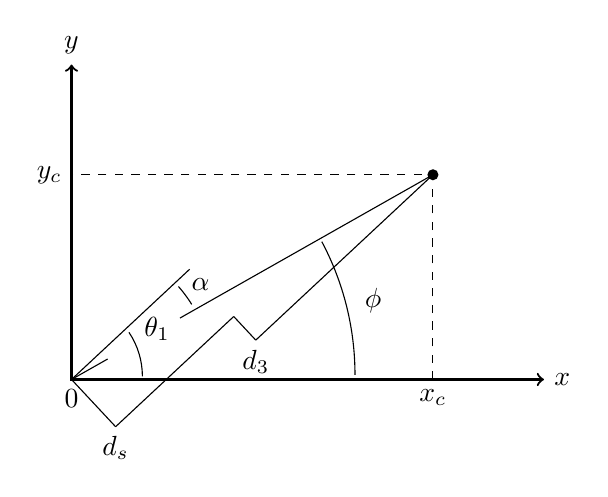
\begin{tikzpicture}[scale=2.0]
	% Draw coordinate axes
	\coordinate[label=below:{$0$}] (origin) at (0,0);
	\draw [<->,thick] (0,2) node (yaxis) [above] {$y$}
		|- (3,0) node (xaxis) [right] {$x$};


	% Desired Point Coordinates	
	\coordinate (xy) at (2.295, 1.3);
	\coordinate[label=below:{$x_c$}](xc) at (2.295,0);
	\coordinate[label=left:{$y_c$}](yc) at (0, 1.3);
	\draw[dashed] (xc) -- (xy) -- (yc);
	\fill[black] (xy) circle (1pt);

	% Theta Angle
	% \coordinate[label=right:{$\alpha$} (thetatarget) at (0.75, 0.7);
	\coordinate (thetatarget) at (0.75, 0.7);
	\coordinate[label=right:{$\theta_1$}] (thetalabel) at (0.4, 0.32);
	\draw (origin) -- (thetatarget);
	\draw (0.45, 0.02) arc (0:34:0.5);
	\draw [black, domain=32:41] plot ({0.9*cos(\x)}, {0.9*sin(\x)});
	\coordinate[label=right:{$\alpha$}] (alphalabel) at (0.7, 0.6);

	% Offset 1
	\coordinate[label=below:{$d_s$}] (ds) at (0.28, -0.3);
	\draw (origin) -- (ds);

	% \coordinate[label=above:{$o_2$}] (o2) at (1.03, 0.4);
	\coordinate (o2) at (1.03, 0.4);
	\draw (ds) -- (o2);

	\coordinate[label=below:{$d_3$}] (d3) at (1.17, 0.25);
	\draw (o2) -- (d3);

	\draw (d3) -- (xy);
	
	% \coordinate (anglestart) at (1.1425, 0.65);
	\draw (0.6885, 0.39) -- (xy);
	\draw (origin) -- (0.2295, 0.13);

	\draw (1.8, 0.03) arc (0:28:1.8);
	\coordinate[label=right:{$\phi$}] (phi) at (1.8, 0.5);
\end{tikzpicture}

From the diagram we can read off:

\begin{align*}
\phi & = Atan2(y_c,x_c)\\
\alpha & = Atan2(d_s + d_3, l_{34} + l_2)\\
\theta_1 & = \phi + \alpha
\end{align*}

Notice that $\alpha$ is a design parameter, but $x_c$ and $y_c$ change.
And the right arm configuration:

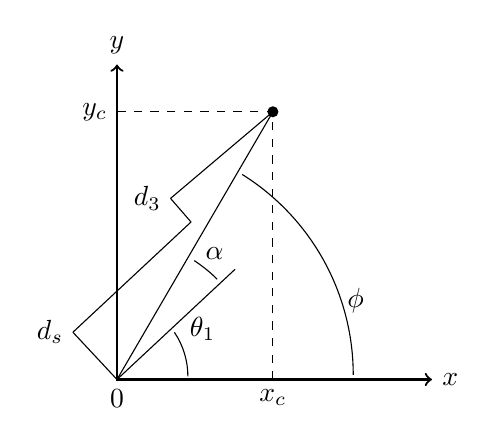
\begin{tikzpicture}[scale=2.0]
	% Draw coordinate axes
	\coordinate[label=below:{$0$}] (origin) at (0,0);
	\draw [<->,thick] (0,2) node (yaxis) [above] {$y$}
		|- (2,0) node (xaxis) [right] {$x$};


	% Desired Point Coordinates	
	\coordinate (xy) at (0.99, 1.7);
	\coordinate[label=below:{$x_c$}](xc) at (0.99,0);
	\coordinate[label=left:{$y_c$}](yc) at (0, 1.7);
	\draw[dashed] (xc) -- (xy) -- (yc);
	\fill[black] (xy) circle (1pt);

	% Theta Angle
	% \coordinate[label=right:{$\alpha$} (thetatarget) at (0.75, 0.7);
	\coordinate (thetatarget) at (0.75, 0.7);
	\coordinate[label=right:{$\theta_1$}] (thetalabel) at (0.4, 0.32);
	\draw (origin) -- (thetatarget);
	\draw (0.45, 0.02) arc (0:34:0.5);
	\draw [black, domain=45:57] plot ({0.9*cos(\x)}, {0.9*sin(\x)});
	\coordinate[label=right:{$\alpha$}] (alphalabel) at (0.5, 0.8);

	% Offset 1
	\coordinate[label=left:{$d_s$}] (ds) at (-0.28, 0.3);
	\draw (origin) -- (ds);

	% \coordinate[label=above:{$o_2$}] (o2) at (1.03, 0.4);
	\coordinate (o2) at (0.47, 1.0);
	\draw (ds) -- (o2);

	\coordinate[label=left:{$d_3$}] (d3) at (0.34, 1.15);
	\draw (o2) -- (d3);

	\draw (d3) -- (xy);
	
	% \coordinate (anglestart) at (1.1425, 0.65);
	\draw (origin) -- (xy);

	\draw (1.5, 0.03) arc (0:58:1.5);
	\coordinate[label=right:{$\phi$}] (phi) at (1.4, 0.5);
\end{tikzpicture}

Where the other two angles are the same as before, but this time:

\begin{align*}
\theta_1 & = \phi - \alpha
\end{align*}

\subsubsection{Determining $\theta_2$ and $\theta_3$}

Now that we've determined $\theta_1$, we can project into a different
	plane to get our values of $\theta_2$ and $\theta_3$.
This will be the plane of the second two joints, which looks like:

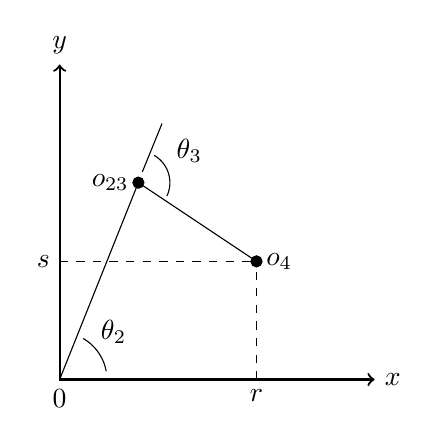
\begin{tikzpicture}[scale=2.0]
	\coordinate[label=below:{$0$}] (origin) at (0,0);
	\draw[<->, thick] (0,2) node (yaxis) [above] {$y$}
		|- (2,0) node (xaxis) [right] {$x$};


	\coordinate[label=left:{$o_{23}$}] (o23) at (0.5, 1.25);
	\draw[black, fill=black] (o23) circle (1pt);
	\draw (origin) -- (o23);

	\coordinate[label=right:{$o_4$}] (o4) at (1.25, 0.75);
	\draw (o23) -- (o4);
	\draw[black, fill=black] (o4) circle (1pt);

	\coordinate[label=below:{$r$}] (r) at (1.25, 0);
	\coordinate[label=left:{$s$}] (s) at (0, 0.75); 
	\draw[dashed] (0, 0.75) -- (o4);
	\draw[dashed] (1.25, 0) -- (o4);

	\draw (0.525, 1.318) -- (0.65, 1.625);
	\coordinate[label=right:{$\theta_3$}] (t3) at (0.68, 1.45);
	\draw [black, domain=-25:60] plot ({0.2*cos(\x) + 0.5},{0.2*sin(\x) + 1.25});

	\draw [black, domain=10:60] plot ({0.3*cos(\x)},{0.3*sin(\x)});
	\coordinate[label=right:{$\theta_2$}] (t2) at (0.2, 0.3);
\end{tikzpicture}


The auxiliary variables $r$ and $s$ correspond to the cylindrical distance
	from the $z_0$ axis $\sqrt{x_c^2 + y_c^2}$, and $s$ is $z_c$.
These are, again, the coordinates of $o_4$ in the frame $o_0 x_0 y_0 z_0$.

In the book, the inverse kinematics of this system are solved.
The solutions are ($D$ is an auxiliary variable):

\begin{align*}
D & = \frac{r^2 + s^2 - l_2^2 - l_{34}^2}{2 l_2 l_{34}} \\
\theta_3 & = Atan2(D, \pm \sqrt{1 - D^2}) \\
\theta_2 & = Atan2(r, s) - Atan2(l_2 + l_{34} \cos \theta_3, l_{34} \sin \theta_3)
\end{align*}

where the choice of $+$ or $-$ corresponds to the choice of the elbow-up
	or elbow-down configuration.

\subsubsection{Summary of Inverse Position}

To achieve a position $o$ with orientation $R$, with respect to an origin
	$o_0 x_0 y_0 z_0$, we can decouple the problem into an inverse position
	problem and an inverse orientation problem.
To attain the orientation $R$ at $o$, the manipulator frame $o_4$
	must be located at:

\[ o_4 = o - d_e R \left[ \begin{matrix} 0\\0\\1\end{matrix} \right] \]

Let $x_c,y_c,z_c$ be the coordinates of $o_4$.
The angles are as follows:

\begin{align*}
\alpha & = Atan2(d_s + d_3, l_{34} + l_2)\\
\phi & = Atan2(y_c, x_c)\\
D & = \frac{r^2 + s^2 - l_2^2 - l_{34}^2}{2 l_2 l_{34}} \\
\theta_1 & = \phi \pm \alpha\\
\theta_2 & = Atan2(r, s) - Atan2(l_2 + l_{34} \cos \theta_3, l_{34} \sin \theta_3) \\
\theta_3 & = Atan2(D, \pm \sqrt{1 - D^2}) \\
\end{align*}

They are determined in the order (1,3,2).
There are two independant choices between positive and negative solutions.
This corresponds to the difference between elbow up, elbow down, 
	and right arm, left arm configurations.
There are therefore four solutions to the inverse position problem.

\subsection{Inverse Orientation Kinematics}

After the inverse position problem has been solved, we need to solve the
	inverse orientation problem.
We have chosen the values of $\theta_1$, $\theta_2$, and $\theta_3$
	to put the arm in a position such that appropriate choices of $\theta_4$,
	$\theta_5$, and $\theta_6$ will put the end-effector frame at $o$ with
	orientation $R$.
We know the position of $o_4$, but we need to determine the orientation
	of the $o_4 x_4 y_4 z_4$ frame so that we can chose angle values
	of $\theta_4, \theta_5, \theta_6$ to put the end-effector in orientation $R$.

We define the rotation of going from frame 0 to frame 3 as $R^0_3$, and the
	totation going from frame 3 to frame 6 as $R^3_6$.
We can determine these rotation matrices from the $A$ matrices:

\[ R^0_3 =
	\left( \begin{matrix}
		c_1 c_2 s_3 + c_1 s_2 c_3 & - s_1 & c_1 c_2 c_3 - c_1 s_2 s_3 \\
		s_1 c_2 s_3 + s_1 s_2 c_3 & c_1 & s_1 c_2 c_3 - s_1 s_2 s_3 \\
		s_2 s_3 & 0 & s_2 c_3 + c_2 s_3 \\
	\end{matrix} \right) \]

\[ R^3_6 = 
	\left( \begin{matrix}
		c_4 s_5 c_6 - s_4 s_6 & -c_4 s_5 s_6 - s_4 c_6 & - c_4 c_5 \\
		s_4 s_5 c_6 + c_4 s_6 & -s_4 s_5 s_6 + c_4 c_6 & - s_4 c_5 \\
		-c_5 c_6 & c_5 s_6 & s_5 \\
	\end{matrix} \right) \]

The goal is to find angles $\theta_4$, $\theta_5$, and $\theta_6$
	such that $R^3_6 = (R_3^0)^{-1} R = (R_3^0)^T R$.

\[	\left( \begin{matrix}
		c_4 s_5 c_6 - s_4 s_6 & -c_4 s_5 s_6 - s_4 c_6 & - c_4 c_5 \\
		s_4 s_5 c_6 + c_4 s_6 & -s_4 s_5 s_6 + c_4 c_6 & - s_4 c_5 \\
		-c_5 c_6 & c_5 s_6 & s_5 \\
	\end{matrix} \right)
	=
	\left( \begin{matrix}
		c_1 c_2 s_3 + c_1 s_2 c_3 & s_1 c_2 s_3 + s_1 s_2 c_3  & s_2 s_3 \\
		 - s_1 & c_1 & 0 \\
		c_1 c_2 c_3 - c_1 s_2 s_3 & s_1 c_2 c_3 - s_1 s_2 s_3  & s_2 c_3 + c_2 s_3 \\
	\end{matrix} \right)
	\left( \begin{matrix}
		r_{11} & r_{12} & r_{13} \\
		r_{21} & r_{22} & r_{23} \\
		r_{31} & r_{32} & r_{33} \\
	\end{matrix} \right)  \]

From the bottom-right, we see:

\begin{align*}
\theta_5 & = \sin^{-1} \left(
		r_{13} ( c_1 c_2 c_3 - c_1 s_2 s_3 ) + r_{23} (s_1 c_2 c_3 - s_1 s_2 s_3)
			+ r_{33} ( s_2 c_3 + c_2 s_3 ) \right) \\
& = \pi - \sin^{-1} \left(
		r_{13} ( c_1 c_2 c_3 - c_1 s_2 s_3 ) + r_{23} (s_1 c_2 c_3 - s_1 s_2 s_3)
			+ r_{33} ( s_2 c_3 + c_2 s_3 ) \right) 
\end{align*}

These are two choices of gripper angle.

Continuing to read off, we see from the middle-right that, assuming $c_5 \neq 0$,

\begin{align*}
\theta_4 & = \frac{\sin^{-1} \left( -s_1 r_{12} + c_1 r_{22} \right) }{- c_5}
\end{align*}

Continuing to read off, we see from the bottom-middle that,
	assuming that $c_5 \neq 0$: 

\begin{align*}
\theta_6 & = \frac{\sin^{-1} \left(
		r_{12} ( c_1 c_2 c_3 - c_1 s_2 s_3 ) + r_{22} (s_1 c_2 c_3 - s_1 s_2 s_3)
			+ r_{32} ( s_2 c_3 + c_2 s_3 ) \right) }{c_5}
\end{align*}

If $c_5 = 0$, then $s_6 = \pm 1$.

Then, from the top-middle and middle-middle entries: 

\begin{align*}
\theta_4 \pm \theta_6 & =
	\cos^{-1} \left( - s_1 r_{12} + c_1 r_{22} \right) \\
\theta_4 \mp \theta_6 & =
	\sin^{-1} \left( \pm \left( (c_1 c_2 s_3 + c_1 s_2 c_3) r_{12}
			+ (s_1 c_2 s_3 + s_1 s_2 c_3) r_{22} + s_2 s_3 r_{32} \right) \right)
\end{align*}

\subsection{Summary}

The PUMA has the following design parameters:

\begin{align*}
l_1 \\
l_2 \\
l_{34} \\
d_s \\
d_3 \\
d_e \\
\end{align*}

To achieve an orientation $R$ and position $o$, we can decouple the 
	problem into an inverse position and inverse orientation problem.
The position problem can be solved first.
We introduce an additional dependant design parameter:

\begin{align*}
\alpha & = Atan2(d_s + d_3, l_{34} + l_2)\\
\end{align*}

We then find the desired coordinates for $o_4$, the center of the
	tool.
These are 

\begin{align*}
o_4 & = o - d_e R \left[ \begin{matrix} 0 \\ 0 \\ 1 \\ \end{matrix} \right]
\end{align*}

Let $ \langle x_c, y_c, z_c \rangle  = o_4$ be the coordinates of $o_4$
	in the base frame $o_0 x_0 y_0 z_0$.

Then, by the geometric approach, we find:

\begin{align*}
\phi & = Atan2(y_c, x_c) \\
\theta_1 & = \phi \pm \alpha\\
\end{align*}

Where this choice of $+$ or $-$ determines whether the arm is in the left-handed
	or right-handed configuration.

Next, we find an auxiliary variable, $D$, by the law of cosines,
	and use it to find $\theta_3$ and then $\theta_2$.

\begin{align*}
D & = \frac{r^2 + s^2 - l_2^2 - l_{34}^2}{2 l_2 l_{34}} \\
\theta_3 & = Atan2(D, \pm \sqrt{1 - D^2}) \\
\theta_2 & = Atan2(r, s) - Atan2(l_2 + l_{34} \cos \theta_3, l_{34} \sin \theta_3) \\
\end{align*}

The choice of $+$ or $-$ here refers to the differnence between an elbow-up
	and elbow-down configuration.

Finally, we find the orientation angles of the rest of the manipulator.

There are two choices of $\theta_5$ orientation, corresponding to the following 
	choices for the value of $\theta_5$:

\begin{align*}
\theta_5 & = \sin^{-1} \left(
		r_{13} ( c_1 c_2 c_3 - c_1 s_2 s_3 ) + r_{23} (s_1 c_2 c_3 - s_1 s_2 s_3)
			+ r_{33} ( s_2 c_3 + c_2 s_3 ) \right) \\
& = \pi - \sin^{-1} \left(
		r_{13} ( c_1 c_2 c_3 - c_1 s_2 s_3 ) + r_{23} (s_1 c_2 c_3 - s_1 s_2 s_3)
			+ r_{33} ( s_2 c_3 + c_2 s_3 ) \right) 
\end{align*}

Once we have determined $\theta_5$, we solve for $\theta_4$ and $\theta_6$.
If $\cos \theta_5 \neq 0$, then:

\begin{align*}
\theta_4 & = \frac{\sin^{-1} \left( -s_1 r_{12} + c_1 r_{22} \right) }{- c_5}\\
& = \frac{\pi - \sin^{-1} \left( -s_1 r_{12} + c_1 r_{22} \right) }{- c_5}
\end{align*}

\begin{align*}
\theta_6 & = \frac{\sin^{-1} \left(
		r_{12} ( c_1 c_2 c_3 - c_1 s_2 s_3 ) + r_{22} (s_1 c_2 c_3 - s_1 s_2 s_3)
			+ r_{32} ( s_2 c_3 + c_2 s_3 ) \right) }{c_5}\\
 & = \frac{\pi - \sin^{-1} \left(
		r_{12} ( c_1 c_2 c_3 - c_1 s_2 s_3 ) + r_{22} (s_1 c_2 c_3 - s_1 s_2 s_3)
			+ r_{32} ( s_2 c_3 + c_2 s_3 ) \right) }{c_5}
\end{align*}

However, if $\cos \theta_5 = 0$, then if $\theta_5 = \frac{\pi}2$:

\begin{align*}
\theta_4 \pm \theta_6 & =
	\cos^{-1} \left( - s_1 r_{12} + c_1 r_{22} \right) \\
\theta_4 \mp \theta_6 & =
	\sin^{-1} \left( \pm \left( (c_1 c_2 s_3 + c_1 s_2 c_3) r_{12}
			+ (s_1 c_2 s_3 + s_1 s_2 c_3) r_{22} + s_2 s_3 r_{32} \right) \right)
\end{align*}
\begin{align*}
\theta_4 & = \frac{ \pm \cos^{-1} \left( - s_1 r_{12} + c_1 r_{22} \right)
		+ \sin^{-1} \left( \left( (c_1 c_2 s_3 + c_1 s_2 c_3) r_{12}
			+ (s_1 c_2 s_3 + s_1 s_2 c_3) r_{22} + s_2 s_3 r_{32} \right) \right)}2\\
& = \frac{ \pm \cos^{-1} \left( - s_1 r_{12} + c_1 r_{22} \right)
		+ \pi -  \sin^{-1} \left( \left( (c_1 c_2 s_3 + c_1 s_2 c_3) r_{12}
			+ (s_1 c_2 s_3 + s_1 s_2 c_3) r_{22} + s_2 s_3 r_{32} \right) \right)}2\\
\theta_6 & = \frac{ \pm \cos^{-1} \left( - s_1 r_{12} + c_1 r_{22} \right)
		- \sin^{-1} \left( \left( (c_1 c_2 s_3 + c_1 s_2 c_3) r_{12}
			+ (s_1 c_2 s_3 + s_1 s_2 c_3) r_{22} + s_2 s_3 r_{32} \right) \right)}2\\
& = \frac{ \pm \cos^{-1} \left( - s_1 r_{12} + c_1 r_{22} \right)
		- \pi +  \sin^{-1} \left( \left( (c_1 c_2 s_3 + c_1 s_2 c_3) r_{12}
			+ (s_1 c_2 s_3 + s_1 s_2 c_3) r_{22} + s_2 s_3 r_{32} \right) \right)}2
\end{align*}

If $\theta_5 = - \frac{\pi}{2}$, then:
\begin{align*}
\theta_4 & = \frac{ \pm \cos^{-1} \left( - s_1 r_{12} + c_1 r_{22} \right)
		+ \sin^{-1} \left( - \left( (c_1 c_2 s_3 + c_1 s_2 c_3) r_{12}
			+ (s_1 c_2 s_3 + s_1 s_2 c_3) r_{22} + s_2 s_3 r_{32} \right) \right)}2\\
& = \frac{ \pm \cos^{-1} \left( - s_1 r_{12} + c_1 r_{22} \right)
		+ \pi -  \sin^{-1} \left( - \left( (c_1 c_2 s_3 + c_1 s_2 c_3) r_{12}
			+ (s_1 c_2 s_3 + s_1 s_2 c_3) r_{22} + s_2 s_3 r_{32} \right) \right)}2\\
\theta_6 & = \frac{ \mp \cos^{-1} \left( - s_1 r_{12} + c_1 r_{22} \right)
		+ \sin^{-1} \left( - \left( (c_1 c_2 s_3 + c_1 s_2 c_3) r_{12}
			+ (s_1 c_2 s_3 + s_1 s_2 c_3) r_{22} + s_2 s_3 r_{32} \right) \right)}2\\
& = \frac{ \mp \cos^{-1} \left( - s_1 r_{12} + c_1 r_{22} \right)
		+ \pi -  \sin^{-1} \left( - \left( (c_1 c_2 s_3 + c_1 s_2 c_3) r_{12}
			+ (s_1 c_2 s_3 + s_1 s_2 c_3) r_{22} + s_2 s_3 r_{32} \right) \right)}2
\end{align*}

I found 5 choices between 2 options, and therefore $32$ solutions.

I have chosen to express the rotation as a rotation matrix.
If the user wishes to use euler angles, then they can find the matrix
	elements with the following formula (Spong 2.27):

\[ \left( \begin{matrix}
	c_\phi c_\theta c_\psi - s_\phi s_\psi &
		-c_\phi c_\theta s_\psi - s_\phi c_\psi &
		c_\phi s_\theta \\
	s_\phi c_\theta c_\psi + c_\phi s_\psi &
		-s_\phi c_\theta s_\psi + c_\phi c_\psi & s_\phi s_\theta \\
	-s_\theta c_\psi & s_\theta s_\psi & c_\theta 
	\end{matrix} \right) \]
	

\end{document}
